これまでにどこかのBBSやブログでご覧になったことがあるかもしれませんが、一つのスレッドや文章の後でいくつもの重複が記録されていることがあります。これらの大多数はユーザが複数回書き込みフォームを送信してしまったことによるものです。様々な原因でユーザはよくフォームを複数回送信してしまいます。通常はマウスの誤操作によるもので、送信ボタンをダブルクリックしてしまったり、一旦送信した内容を再度修正しようとして、ブラウザの戻るボタンを押した後に次へボタンではなくまた送信ボタンを押してしまうことによるものです。当然、故意によるものもあります。- - 例えばネット上のアンケート調査やくじ引きにおいて重複して投票するなどです。では、どのようにしてユーザが同じ内容のフォームの送信を行うことを効果的に防げるのでしょうか?

解決方法はフォームの中にユニークな値を持ったhiddenフィールドを追加することです。フォームを検証する際、このユニークな値を持ったフォームがすでに送信されているかどうか検証します。もしすでに送信されていれば、二回目の送信を拒絶します。そうでなければフォームに対して処理ロジックを行います。また、もしAjax形式で送信するフォームだった場合、フォームが送信された後javascriptによってフォームの送信ボタンを禁止します。

4.2節の例を改良してみましょう:

\begin{lstlisting}[numbers=none]
<input type="checkbox" name="interest" value="football">サッカー
<input type="checkbox" name="interest" value="basketball">バスケットボール
<input type="checkbox" name="interest" value="tennis">テニス
ユーザ名:<input type="text" name="username">
パスワード:<input type="password" name="password">
<input type="hidden" name="token" value="{{.}}">
<input type="submit" value="ログイン">
\end{lstlisting}

テンプレートの中に\texttt{token}というhiddenフィールドを追加しました。この値にはMD5(タイムスタンプ)によってユニークな値を割り当てます。この値をサーバに保存することで(sessionによるコントロールは6章でどのように保存するか解説します)フォームが送信される際の判定に使うことができます。

\begin{lstlisting}[numbers=none]
func login(w http.ResponseWriter, r *http.Request) {
    fmt.Println("method:", r.Method) //リクエストを受け取る方法
    if r.Method == "GET" {
        crutime := time.Now().Unix()
        h := md5.New()
        io.WriteString(h, strconv.FormatInt(crutime, 10))
        token := fmt.Sprintf("%x", h.Sum(nil))

        t, _ := template.ParseFiles("login.gtpl")
        t.Execute(w, token)
    } else {
        //リクエストはログインデータです。
        //ログインのロジックを実行して判断します。
        r.ParseForm()
        token := r.Form.Get("token")
        if token != "" {
            //tokenの合法性を検証します。
        } else {
            //tokenが存在しなければエラーを出します。
        }
        fmt.Println("username length:",
                    len(r.Form["username"][0]))
        fmt.Println("username:",
                    template.HTMLEscapeString(r.Form.Get("username")))
        //サーバ側に出力します。
        fmt.Println("password:",
                    template.HTMLEscapeString(r.Form.Get("password")))
        template.HTMLEscape(w, []byte(r.Form.Get("username")))
        //クライアントに出力します。
    }
}
\end{lstlisting}

出力されるページのソースは以下の通り:

\begin{figure}[H]
  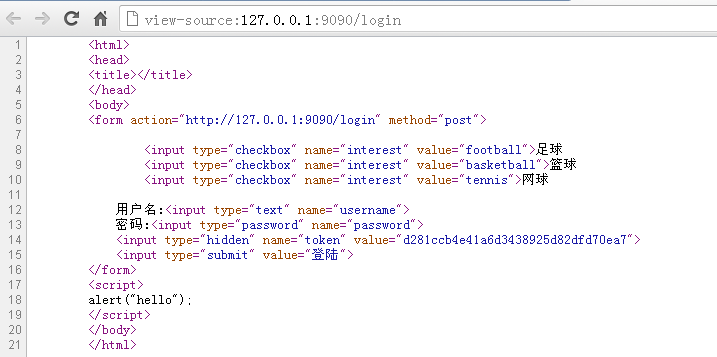
\includegraphics[width=14cm]{4.4.token.png}
   \label{図4.4}
   \caption{tokenを追加した後クライアントが出力するソース情報}
\end{figure}

tokenはすでに出力値を持っていますので連続してページを更新することができます。この値が次々と変化するのがお分かりいただけるかと思います。このように毎回formが表示される時にユニークになるよう保証します。ユーザが送信するフォームは唯一性が保持されます。

この解決方法は悪意の無い攻撃に対しても防止することができます。また悪意のあるユーザに対してもしばらく効果があります。その後、ユーザーにこの悪意のある動機を捨てさせることができなかった場合は更に複雑な作業が必要となります。
